\documentclass[oneside, article]{memoir}

% \usepackage{bibte?}
% \addbibresource{measurement-error-gp.bib}

\usepackage{lmodern}
\usepackage{amsmath, amsthm, amsfonts, amssymb, mathtools, commath,
hyperref, cancel, bm}
\usepackage{doi, xcolor}
% \usepackage[T1]{fontenc}

% \usepackage{eulervm}
\usepackage[tracking, spacing]{microtype}
\usepackage[margin=1in]{geometry}
\microtypecontext{spacing=nonfrench}
\newtheorem{definition}{Definition}
\newtheorem{proposition}{Proposition}
\newtheorem{conjecture}{Conjecture}
\newtheorem{theorem}{Theorem}
\newtheorem{problem}{Problem}
\newtheorem{corollary}{Corollary}
\newtheorem{remark}{Remark}
\newtheorem{lemma}{Lemma}
\newtheorem{example}{Example}
\DeclareMathOperator{\trace}{\operatorname{tr}}
\DeclareMathOperator{\expect}{\mathbb{E}}
\DeclareMathOperator{\probability}{\mathbb{P}}
\DeclareMathOperator{\Var}{\operatorname{Var}}
\DeclareMathOperator{\Cov}{\operatorname{Cov}}
\begin{document}
Analytic filtering for single-layer RBF dynamics:
\cite{deisenroth_analytic_2009}
\chapter{MMSE filtering background}
Suppose that the nominal system dynamics are given by
% \begin{subequations}
\begin{align}
  x_{t+1} &= F(x_{t}, u_t) + \eta_t \\
  y_t &= H(x_t, u_t) + \epsilon_t
  \intertext{
    where \(F\) and \(H\) are nonlinear functions, \(u_t\) is exogeneous input, and \(\eta_t\) and \(\epsilon_t\) are white noise processes.
    The vanilla MMSE linear filter (with no simplifications except for the gausssian variational Ansatz of Assumed Density Filtering) has two steps, \textbf{predict}:
  }
    % \xi_{t-1} &\sim \mathcal{N}(\hat x_{t-1 \mid t-1}, P^{xx}_{t-1 \mid t-1})
  % \tag{MaxEnt approximation}
  % \\
  \hat x_{t\mid t - 1}
  &= \expect_{\xi \sim \mathcal{N}(\hat x_{t-1 \mid t-1}, P^{xx}_{t-1 \mid t-1})}
  F(\xi, u_{t-1})
  % \tag{mean}
  \\
  \hat P^{xx}_{t\mid t - 1}
  &= \Var_{\xi \sim \mathcal{N}(\hat x_{t-1 \mid t-1}, P^{xx}_{t-1 \mid t-1})}
  F(\xi, u_{t-1}) + Q
  \\
  % \hat 
  \hat y_{t \mid t-1}
  &= \expect_{\xi \sim \mathcal{N}(\hat x_{t \mid t-1}, P^{xx}_{t \mid t-1})}
   H(\hat x_{t \mid t-1}, u_t)
  \\
  \hat P^{xy}_{t \mid t-1}
  &= \Cov_{
    \xi \sim \mathcal{N}(\hat x_{t \mid t-1}, P^{xx}_{t \mid t-1})
  }
   (\xi, H(\hat x_{t \mid t-1}, u_t))
  \\
  \hat P^{yy}_{t \mid t-1}
  &= \Var_{
    \xi \sim \mathcal{N}(\hat x_{t \mid t-1}, P^{xx}_{t \mid t-1})
  }
   H(\xi, u_t)
   + R
  \\
  \intertext{and \textbf{update}:}
  \hat x_{t \mid t}
  &= \hat x_{t \mid t-1} + \hat P^{xy}_{t \mid t-1} \del{\hat P^{yy}_{t\mid t-1}}^{-1} (y_t - \hat y_{t \mid t-1})
  \tag{conditional mean}
  \\
  \intertext{(optionally iterate these covariances using \(\hat x_{t\mid t}\))}
  \hat P^{xx}_{t \mid t}
  &= \hat P^{xx}_{t \mid t-1} - \hat P^{xy}_{t \mid t-1} \del{\hat P^{yy}_{t\mid t-1}}^{-1} \del{\hat P^{xy}_{t \mid t-1}}^\intercal
  \tag{conditional covariance}
\end{align}

The next step is to decide how to compute the first and second moments of \(F(\xi_{t-1}, u_{t})\), which have explicit formulas if \(F\) is linear.
Otherwise,
one may approximate \(F\) by its linearization (EKF) or approximate the law of \(\xi_{t-1}\) by a discrete distribution (UKF).
They have their strengths and weaknesses.

In this note, I show that if \(F\) is a neural network with one hidden layer, there is an analytic expression for these moments.
A Gaussian mean and covariance can be propagated analytically through a sigmoid-plus-linear layer.
After this nonlinear transformation, we impose a variational approximation that the output is Gaussian.
This approximation can be justified heuristically on the basis of maximum entropy.
It is plausible to extend this approximation to deep networks.

\chapter{Analytic moments of neural networks}
Neural networks are compositions of \emph{layers}, where each layer is an affine functions followed by an elementwise nonlinearity.
They are popular because folk wisdom has found that composition can be a more effective parameterization for function approximation than, say, addition, or interpolation.
A typical nonlinear layer looks like:
\begin{align}
  f(x; A, b, C, d) &= \sigma(A x + b) + Cx + d
  \label{eq:layer}
  \intertext{where \(A, b, C, d\) are learnable parameters, and \(\sigma\) is a nonlinearity.
  In the rest of this note, I will take \(\sigma = 2\Phi - 1\), where \(\Phi\) is the standard Normal CDF:}
  \sigma(t) &:= 2\Phi(t) - 1
  =
  \sqrt{\frac{2}{\pi}} \int_{0}^t e^{-\frac{1}{2} u^2} du.
\end{align}
For ease of notation, I will work out these computations for the case where \(A = a^\intercal\) and \(C=c^\intercal\) are row vectors, and \(b\) and \(d\) are scalars.
It will be fairly simple to extend row-wise to matrix-valued \(A,b, C, d\).

\begin{remark}
  The methods in this note generalize to arbitrary \(\sigma\) as long as there are analytic or numerical (e.g.~polynomial or LUT) approximations to \(\expect \sigma(X) \sigma(Y)\) and \(\expect \sigma (X) Y\) where \(X\) and \(Y\) are jointly Normal.
  I am only using \(\Phi\) because it lends itself well to closed-form expressions.\footnote{It also depends on what you count as closed form. The 1D normal CDF is a common ``special function.'' But I had to do some work to get a numerical approximation to the bivariate normal CDF.}
\end{remark}


\begin{lemma}
  Let \(X \sim \mathcal N(\mu, \Sigma)\).
  % and let \(f\) be as in \eqref{eq:layer}.
  Then
  \begin{align*}
    M(\mu, \Sigma; a, b, c, d) :=
    \expect f(X; a, b, c, d) &= 
    \sigma\del{\frac{b + a^\intercal \mu}{\sqrt{1 + a^\intercal \Sigma a}}}
    + c^\intercal \mu + d
  \end{align*}
  \label{lem:mean}
\end{lemma}
\begin{proof}
  % In indices.
  \begin{align}
    \expect f(X; a, b, c, d)
    &= -1+2\expect \Phi\del{a^\intercal X + b} + c^\intercal \mu + d
    \\
    &= -1+2\expect \probability \sbr{{Z \leq a^\intercal X + b} \mid X} + c^\intercal \mu + d
    \tag{introducing an independent \(Z \sim \mathcal{N}(0, 1)\)}
    \\
    &= -1+2\probability\sbr{{Z \leq a^\intercal X + b}} + c^\intercal \mu + d
    \tag{by the law of total probability}
    \\
    &= -1+2\probability \sbr{{Z - a^\intercal X \leq b}} + c^\intercal \mu + d
    \intertext{The random variable \(Z - a^\intercal X\) has a Normal distribution with mean \(-a^\intercal \mu\) and variance \(1 + a^\intercal \Sigma a\), so}
    \probability \sbr{\bm{1}_{Z - a^\intercal X \leq b}}
    &= \Phi\del{\frac{b + a^\intercal \mu}{\sqrt{1 + a^\intercal \Sigma a}}}.
    % \intertext{In matrix-vector form, we have}
  \end{align}
  % The conclusion follows from converting back to matrix-vector form with an elementwise nonlinearity.
\end{proof}

\begin{lemma}
  Let \(X \sim \mathcal N(\mu, \Sigma)\).
  % and let \(f\) be as in \eqref{eq:layer}.
  Then
  \begin{align*}
    K(\mu, \Sigma; a_1, b_1, c_1, d_1, a_2, b_2, c_2, d_2)
    &:= \Cov (f(X; a_1, b_1, c_1, d_1), f(X; a_2, b_2, c_2, d_2) )
    \\
    \begin{split}
      &= 
      4\Phi_2\del{
        \frac{\mu_1}{\sigma_1},
        \frac{\mu_2}{\sigma_2};
        \frac{a_1^\intercal \Sigma a_2}{
          \sigma_1\sigma_2
        }
      } - 4\Phi\del{\frac{\mu_1}{\sigma_1}} \Phi\del{\frac{\mu_1}{\sigma_2}}
      \\
      &\quad +
      2\frac{a_1^\intercal \Sigma c_2} {\sigma_1} 
      \phi\del{\frac{\mu_1}{\sigma_1}}
      \\
      &\quad+
      2\frac{a_2^\intercal \Sigma c_1}{\sigma_2} 
      \phi\del{
        \frac{\mu_2}{\sigma_2} 
        }
      \\
      &\quad
      +c_1^\intercal \Sigma c_2,
    \end{split}
  \intertext{where }
    \mu_1 &= a_1^\intercal \mu + b_1,
    \\  
    \mu_2 &= a_2^\intercal \mu + b_2,
    \\
    \sigma_1 &= \sqrt{1 + a_1^\intercal \Sigma a_1},
    \\
    \sigma_2 &= \sqrt{1 + a_2^\intercal \Sigma a_2},
    \\
  \end{align*}
  and \(\phi = \Phi'\) and \(\Phi_2(\cdot, \cdot; \rho)\) is the bivariate normal CDF with standard deviation 1 and correlation \(\rho\).
\end{lemma}
\begin{proof}
  The constant terms \(-1+d\) can be dropped.
  Substituting the remaining terms of \(f\), we have
  % A formula for the covariance of asum reads
  \begin{multline}
    \Cov (f(X; a_1, b_1, c_1, d_1), f(X; a_2, b_2, c_2, d_2) )
    \\
    =
    4\underbrace{\Cov(\Phi(a_1^\intercal x + b_1), \Phi(a_2^\intercal x + b_2))}_{K_1} 
    +2\underbrace{\Cov(\Phi(a_1^\intercal x + b_1), c_2^\intercal x)}_{K_2} 
    +2\underbrace{\Cov(\Phi(a_2^\intercal x + b_2), c_1^\intercal x)}_{K_3} 
    +\underbrace{\Cov(c_1^\intercal x, c_2^\intercal x)}_{K_4} 
  \end{multline}
  By a similar calculation as in Lemma~\ref{lem:mean}, we introduce \(Z_1, Z_2 \sim \mathcal N(0, 1)\) and have
  \begin{align}
    % K_1 &=
    % \expect \Phi(a_1^\intercal X + b_1) \Phi(a_2^\intercal X + b_2)
    % - \expect \Phi(a_1^\intercal X + b_1) \expect \Phi(a_2^\intercal X + b_2)
    % \\
    % &= 
    \expect \Phi(a_1^\intercal X + b_1) \Phi(a_2^\intercal X + b_2)
    &= 
    \expect \expect\sbr{
      \bm1_{Z_1 - a_1^\intercal X \leq b_1} \mid X
    }
    \expect\sbr{
      \bm1_{Z_2 - a_2^\intercal X \leq b_2} \mid X
    }
    \\
    &= 
    \expect \expect\sbr{
      \bm1_{Z_1 - a_1^\intercal X \leq b_1} \bm1_{Z_2 - a_2^\intercal X \leq b_2} \mid X
    }
    \\
    &= 
    \probability\sbr{
      Z_1 - a_1^\intercal X \leq b_1, Z_2 - a_2^\intercal X \leq b_2
    }
    \label{eq:joint-prob}
  \end{align}
  Because the random vector \((Z_1 - a_1^\intercal X, Z_2 - a_2^\intercal X)\) has a multivariate normal distribution
  \begin{align}
    \begin{pmatrix}
      Z_1 - a_1^\intercal X
      \\
      Z_2 - a_2^\intercal X
    \end{pmatrix}
    \sim
    \mathcal{N}\del{
      \begin{pmatrix}
        -a_1^\intercal \mu
        \\
        -a_2^\intercal \mu
      \end{pmatrix},
      \begin{pmatrix}
        1 + a_1^\intercal \Sigma a_1
        &
        a_1^\intercal \Sigma a_2
        \\
        a_2^\intercal \Sigma a_1
        &
        1 + a_2^\intercal \Sigma a_2
      \end{pmatrix}
    },
  \end{align}
  the probability \eqref{eq:joint-prob} is
  \begin{align}
    \probability\sbr{
      Z_1 - a_1^\intercal X \leq b_1, Z_2 - a_2^\intercal X \leq b_2
    }
    &= \Phi_2\del{
      \frac{\mu_1}{\sigma_1},
      \frac{\mu_2}{\sigma_2};
      \frac{a_1^\intercal \Sigma a_2}{
        \sigma_1\sigma_2
      },
    }
  \end{align}
  Thus
  \begin{align}
    K_1 &= \expect \Phi(a_1^\intercal X + b_1) \Phi(a_2^\intercal X + b_2) - \expect \Phi(a_1^\intercal X + b_1) \expect \Phi(a_2^\intercal X + b_2) \\
    &= \Phi_2\del{
      \frac{\mu_1}{\sigma_1},
      \frac{\mu_2}{\sigma_2};
      \frac{a_1^\intercal \Sigma a_2}{
        \sigma_1\sigma_2
      }
    } - \Phi\del{\frac{\mu_1}{\sigma_1}} \Phi\del{\frac{\mu_1}{\sigma_2}}
  \end{align}

  Now to compute \(K_2\).
  Notice that \((a_1^\intercal x + b, c_2^\intercal x)\) has the same distribution as 
  \begin{align}
    \begin{pmatrix}
      \zeta_1
      \\
      \zeta_2
    \end{pmatrix}
    \sim
    \mathcal{N}\del{
      \begin{pmatrix}
        a_1^\intercal \mu + b_1
        \\
        c_2^\intercal \mu
      \end{pmatrix},
      \begin{pmatrix}
        1 + a_1^\intercal \Sigma a_1
        &
        a_1^\intercal \Sigma c_2
        \\
        a_1^\intercal \Sigma c_2
        &
        1 + c_2^\intercal \Sigma c_2
      \end{pmatrix}
    }
  \end{align}
  Therefore, by Stein's lemma,
  \begin{align}
    \Cov (\Phi(a_1^\intercal x + b_1), c_2^\intercal x)
    = 
    \Cov (\Phi(\zeta_1), \zeta_2)
    &= \Cov\del{\zeta_1, \zeta_2} \expect \phi(\zeta_1)
    \\
    &= 
    (a_1^\intercal \Sigma c_2) \expect \phi(\zeta_1).
    \label{eq:K2-intermediate}
  \end{align}
  % where \(\phi = \Phi'\).
  This latter expectation may be computed using the formula
  \begin{align}
    \expect \phi(Z)
    &= \frac{1}{\sqrt{1 + \sigma_Z^2}} \phi\del{\frac{\mu_ Z}{\sqrt{1 + \sigma_Z^2}}}
    % &= \frac{1}{\sigma_1}
    % \int_\mathbb{R} \phi(\zeta_1) \phi\del{\frac{\zeta_1 - (a_1^\intercal \mu + b_1)}{\sigma_1}} \dif \zeta_1
    % \\
    % &= 
    % \frac{\sqrt{\sigma_1^2 + 1}}{\sigma_1} \phi\del{
    %   \frac{\sqrt{\sigma_1^2 + 1}}{\sigma_1}
    %   \del{a_1^\intercal \mu + b_1}
    % }
  \end{align}
  when \(Z \sim \mathcal N(\mu_Z, \sigma_Z^2)\).
  Combining with \eqref{eq:K2-intermediate} yields
  \begin{align}
    K_2
    &= 
    \del{a_1^\intercal \Sigma c_2} 
    \frac{1}{\sqrt{1 + a_1^\intercal \Sigma a_1}} 
    \phi\del{\frac{\mu_1}{\sqrt{1 + a_1^\intercal \Sigma a_1}}}
    \intertext{Likewise, with 1s and 2s reversed,}
    K_3
    &= 
    \del{a_2^\intercal \Sigma c_1}
    \frac{1}{\sqrt{1 + a_2^\intercal \Sigma a_2}} 
    \phi\del{
      \frac{\mu_2}{\sqrt{1 + a_2^\intercal \Sigma a_2}} 
      }
  \end{align}
  Finally,
  \begin{align}
    K_4 &= c_1^\intercal \Sigma c_2.
  \end{align}
\end{proof}

\clearpage
\chapter{Numerical example}
With random \((A, b, C, d)\)s, I prepared a deepish MLP with
\begin{itemize}
  \item 2-dimensional input \(x \sim \mathcal N(0, \alpha I)\) and.
  \item 1-dimensional output \(y\)
\end{itemize}
defined by
\begin{align}
  y = \del{f_4 \circ f_3 \circ f_2 \circ f_1}(x)
\end{align}
where all the intermediate layers have 10 neurons.
The figure on the next page shows Monte Carlo results (100,000 repetitions) for \(\alpha \in (0.01, 1, 100)\):
\begin{description}
  \item[empirical KDE]  is a kernel density estimate of the true distribution of \(y\)
  \item[pseudo-true Gaussian fit] is a Gaussian PDF parameterized by the sample mean and variance of \(y\)
  \item[unscented approximation] is the Unscented Transform applied to \(\del{f_4 \circ f_3 \circ f_2 \circ f_1}\) with untuned default settings.
  \item[linear approximation] is a small-variance delta method formula similar to what EKF uses
  \item[my approximation] is my formula applied to Gaussian re-approximations at the output of each layer.
\end{description}
The goodness of approximation at \(\alpha=100\) suggests that my formula might be good for high-\(Q\) nonlinear filtering applications.

% \begin{figure*}
\clearpage
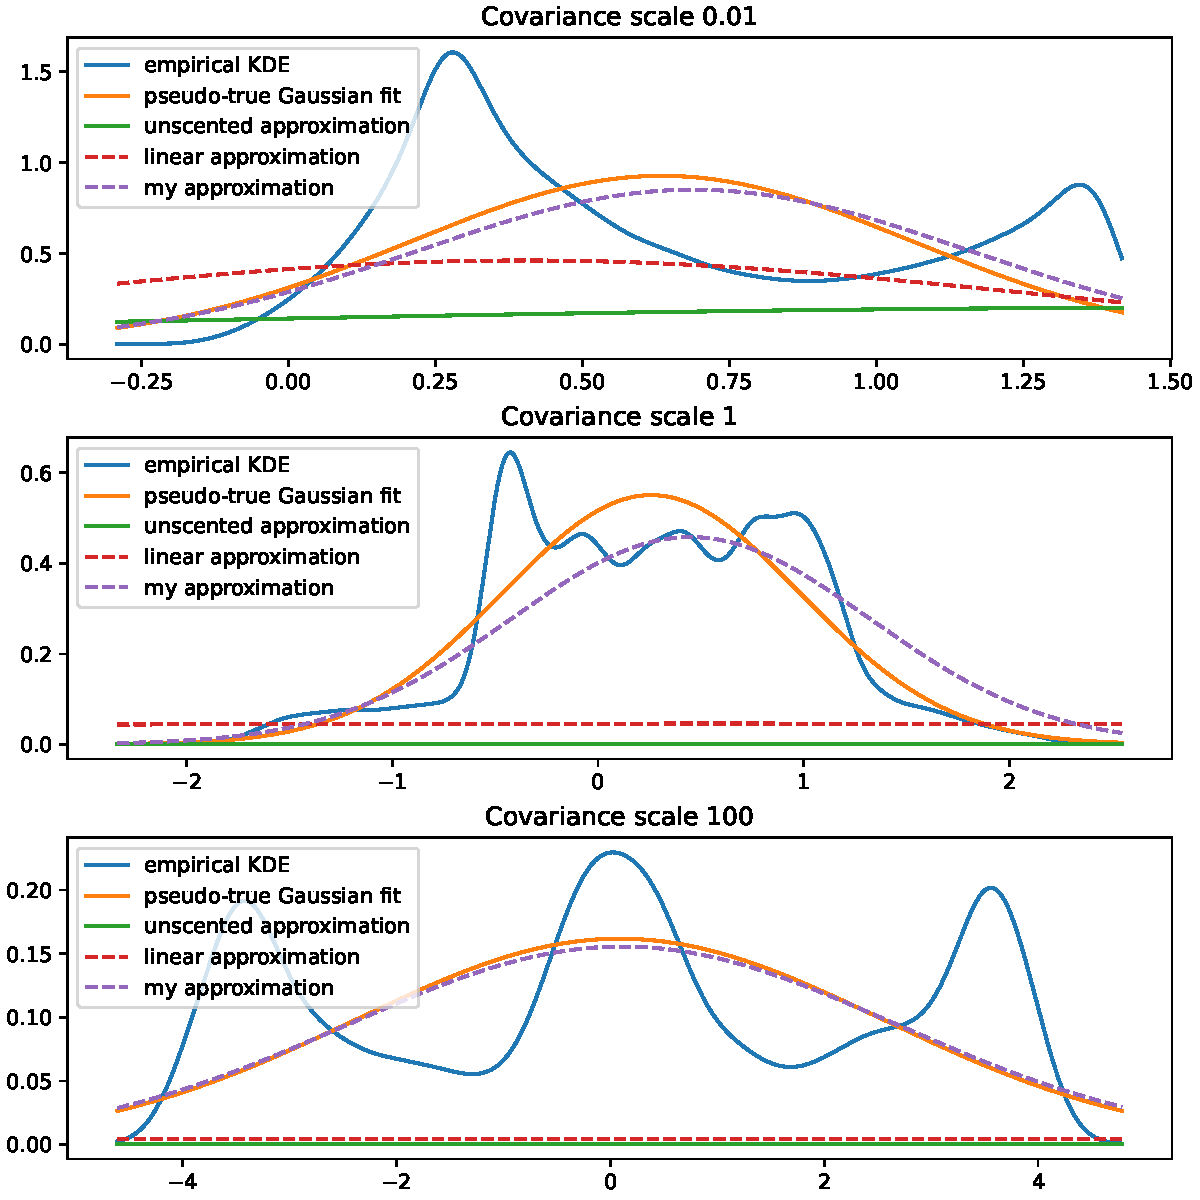
\includegraphics[width=\textwidth]{../figures/deep-mlp.pdf}
%   \caption{\label{fig:deep-mlp}}
% \end{figure*}
\bibliographystyle{abbrv}
\bibliography{nn-filtering}
\end{document} 